\documentclass[border=5pt]{standalone}
\usepackage[T1]{fontenc}
\usepackage{tikz}
\usetikzlibrary{positioning, arrows.meta, decorations.pathreplacing, calc}

\begin{document}

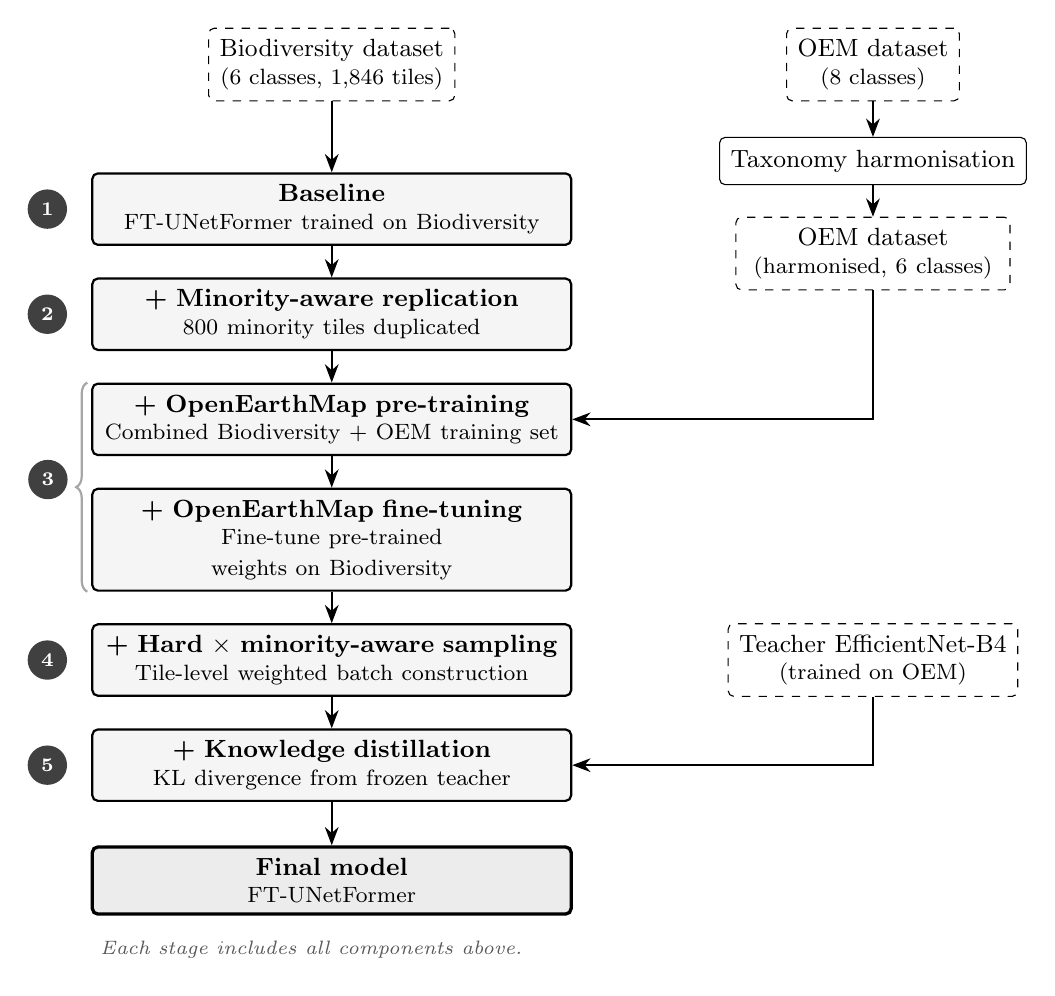
\begin{tikzpicture}[
  font=\small,
  >=Stealth,
  % --- node styles ---
  data/.style={
    draw, dashed, rounded corners=2pt,
    minimum height=0.6cm, align=center, inner sep=4pt
  },
  proc/.style={
    draw, rounded corners=2pt,
    minimum height=0.6cm, align=center, inner sep=4pt
  },
  stage/.style={
    proc, thick, fill=gray!8, text width=5.8cm
  },
  final/.style={
    proc, very thick, fill=gray!15, text width=5.8cm
  },
  snum/.style={
    circle, fill=black!75, text=white,
    font=\scriptsize\bfseries,
    inner sep=0pt, minimum size=5mm
  },
  snumsm/.style={
    snum, font=\tiny\bfseries, inner sep=0pt, minimum size=5mm
  },
  arr/.style={->, thick},
]

% ══════════════════════════════════════════════
% DATA SOURCES (top)
% ══════════════════════════════════════════════

\node[data] (bio) {Biodiversity dataset\\[-1pt]
  {\footnotesize (6 classes, 1,846 tiles)}};

\node[data, right=4.2cm of bio] (oem) {OEM dataset\\[-1pt]
  {\footnotesize (8 classes)}};

\node[proc, below=0.45cm of oem] (tax) {Taxonomy harmonisation};

\node[data, below=0.4cm of tax, text width=3.2cm] (oem6) {OEM dataset\\[-1pt]
  {\footnotesize (harmonised, 6 classes)}};

\draw[arr] (oem) -- (tax);
\draw[arr] (tax) -- (oem6);

% ══════════════════════════════════════════════
% MAIN PIPELINE
% ══════════════════════════════════════════════

\node[stage, below=0.9cm of bio] (s1) {
  \textbf{Baseline}\\[-1pt]
  {\footnotesize FT-UNetFormer trained on Biodiversity}};
\node[snum, left=3mm of s1] {1};

\node[stage, below=0.4cm of s1] (s2) {
  \textbf{+ Minority-aware replication}\\[-1pt]
  {\footnotesize 800 minority tiles duplicated}};
\node[snum, left=3mm of s2] {2};

\node[stage, below=0.4cm of s2] (s3a) {
  \textbf{+ OpenEarthMap pre-training}\\[-1pt]
  {\footnotesize Combined Biodiversity + OEM training set}};

\node[stage, below=0.4cm of s3a] (s3b) {
  \textbf{+ OpenEarthMap fine-tuning}\\[-1pt]
  {\footnotesize Fine-tune pre-trained weights on Biodiversity}};

\node[stage, below=0.4cm of s3b] (s4) {
  \textbf{+ Hard} $\times$ \textbf{minority-aware sampling}\\[-1pt]
  {\footnotesize Tile-level weighted batch construction}};
\node[snum, left=3mm of s4] {4};

\node[stage, below=0.4cm of s4] (s5) {
  \textbf{+ Knowledge distillation}\\[-1pt]
  {\footnotesize KL divergence from frozen teacher}};
\node[snum, left=3mm of s5] {5};

\node[final, below=0.55cm of s5] (fin) {
  \textbf{Final model}\\[-1pt]
  {\footnotesize FT-UNetFormer}};

% ══════════════════════════════════════════════
% MAIN FLOW ARROWS
% ══════════════════════════════════════════════

\draw[arr] (bio) -- (s1);
\draw[arr] (s1) -- (s2);
\draw[arr] (s2) -- (s3a);
\draw[arr] (s3a) -- (s3b);
\draw[arr] (s3b) -- (s4);
\draw[arr] (s4) -- (s5);
\draw[arr] (s5) -- (fin);

% ══════════════════════════════════════════════
% CROSS-DATASET INPUTS
% ══════════════════════════════════════════════

% OEM → Stage 3a
\draw[arr] (oem6.south) |- (s3a.east);

% Teacher → Stage 5
\node[data] at (oem6 |- s4) (teacher) {Teacher EfficientNet-B4\\[-1pt]
  {\footnotesize (trained on OEM)}};
\draw[arr] (teacher.south) |- (s5.east);

% ══════════════════════════════════════════════
% STAGE 3 BRACE
% ══════════════════════════════════════════════

\draw[decorate,
  decoration={brace, amplitude=4pt, mirror},
  thick, gray!70]
  ([xshift=-0.5mm]s3a.north west) -- ([xshift=-0.5mm]s3b.south west);

% Stage-3 number, circled and column-aligned with stages 1/2/4/5;
% the brace sits just left of the boxes and its nub points at this circle.
\node[snum] at ([xshift=-5.5mm]$(s3a.west)!0.5!(s3b.west)$) {3};

% ══════════════════════════════════════════════
% ANNOTATION
% ══════════════════════════════════════════════

\node[font=\scriptsize\itshape, text=black!65, anchor=north west]
  at ([yshift=-2mm]fin.south west)
  {Each stage includes all components above.};

\end{tikzpicture}

\end{document}
